
\section{Software Architecture}
Because we are using nxtOSEK as our operating system for the bus \todo{has this been decided at this point in the report??, if not, then write it here}, we can program using either C or C++, see \ref{nxtOSEK} for more details. Because we can split the program cleanly into modular components as shown in the diagram \ref{fig:components}, we will program using the object-oriented programming paradigm in C++. 

Using the separated components as the baseline, we now create a class diagram that is less abstract than the component separation, which we will use as the software architecture of our model (the programming logic of the bus) implementation. Using this diagram, we will later create precise interfaces for all its classes. The dark blue boxes signify the physical sensors that the program will need to communicate with. 

The arrows on the figure signify function calls, e.g. if an arrow points from object A to B, it means that object A will call functions from object B. To better describe the concerns of each class on the diagram, we've written an example of one function call that might occur between the objects on each edge. This part isn't intended to be extremely precise, however, it helps communicate how we are planning to use object-oriented programming for information hiding and abstraction. See the diagram on \ref{fig:softwareArchitecture}

\begin{figure}[ht]
    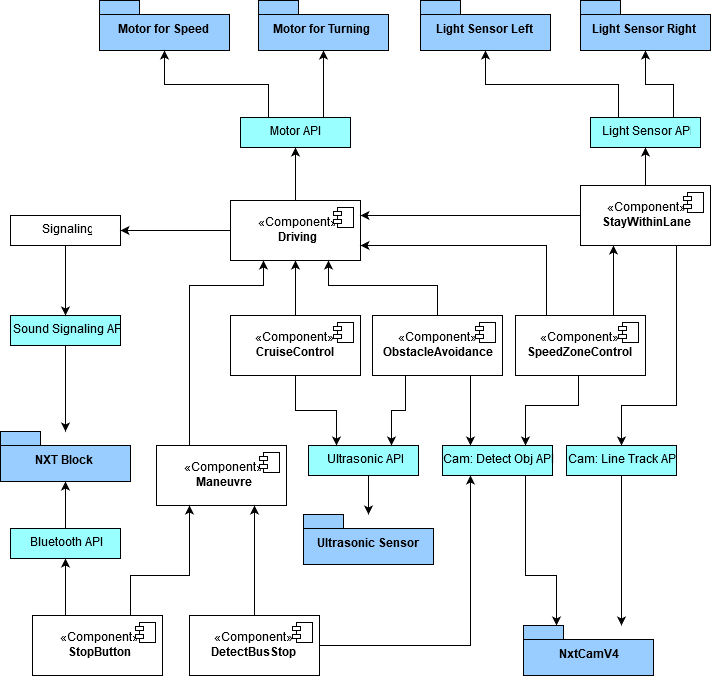
\includegraphics[width=\textwidth]{Images/Design/architectureClassDiagram.png}
    \caption{Class diagram of the program architecture of the model; function call examples are written on the edges}
    \label{fig:softwareArchitecture}
\end{figure}

The intent is that we use this diagram directly for our program architecture, so that each object on the diagram becomes a class in the implementation. The light blue coloured API-objects are also classes that we will create ourselves. The point with these is that they expose the useful functions that each sensor/actuator has, while also automatically filtering out incorrect measurements and calibrating the sensors.
%The figure above shows the implementation of our model, ie. the software of the bus that we write ourselves.

Do, however, note that the diagram is still a bit of a simplification. Specifically, the sensor API classes do not communicate directly with their corresponding sensors; instead they all query the NXT block, that gives access to different functions dependant on which sensors are connected. The diagram simply shows the model of the program, so we don't wish to directly deal with these sorts of implementation and low-level details. 

Something to note, which is not mentioned on the diagram, is that we have also planned to write a program separate from the system, which has the one job of sending messages via bluetooth to the NXT-block whenever we wish to illustrate that a passenger has clicked the stop-button. This is intended to work just like a stub-function would, and the rest of the program simply pretends that a real passenger clicked a button inside the bus.

